\clearpage

\section{Konkurrentanalyse}

Målet med konkurrentanalysen er å finne inspirasjon og kunnskap til nettstedet vi skal utvikle, ved å se på allerede eksisterende løsninger. Hvem er oppdragsgiver sine konkurrenter? Hvordan type løsning har disse valgt? Hvilke styrker og svakheter har løsningene? Analysen er først og fremst gjort fra en vanlig bruker sitt perspektiv, men noen tekniske faktorer har også blitt vurdert.

\subsection{Teknisk analyse}
For å vurdere de tekniske faktorene har vi brukt Google Lighthouse til å sjekke hvor raskt nettstedene laster inn, beste praksis og SEO. I tillegg ble WAVE \footnote{Web Accessibility Evulation Tool. http://wave.webaim.org/} brukt til å sjekke om nettstedene følger kravene for loven om universell utforming og tilgjengelighet.

\subsection{Konkurrentene}
Sirkus Media har mange konkurrenter, deriblant alle firmaer som driver mediebyråvirksomhet. Etter samtale med Hans Christian Hymer \footnote{Samtale med oppdragsgiver (16.01.2019)} fikk vi oppgitt 3 bedrifter som blir ansett som Sirkus Media sine største konkurrenter. Det er følgelig disse konkurrentene vi har valgt å analysere.

\subsection{TACTIC™ Real-Time Marketing}
Nettstedet til TACTIC™ Real-Time Marketing ligger på følgende domene; https://tacticrealtime.com

\subsubsection{Førsteinntrykk}
Førsteinntrykket er at nettstedet fremstår ryddig og profesjonelt. Det første som møter deg er et stort bakgrunnsbilde. Bilde dekker hele skjermen og har en tittel og en underoverskrift. Headeren består også av en knapp der du kan trykke på \q{Request a demo}. Helt øverst på forsiden er logoen til Tactic og en meny. Til høyre er det en knapp som gir deg muligheten til å se på en video. 

\begin{figure}[H]
    \centering
    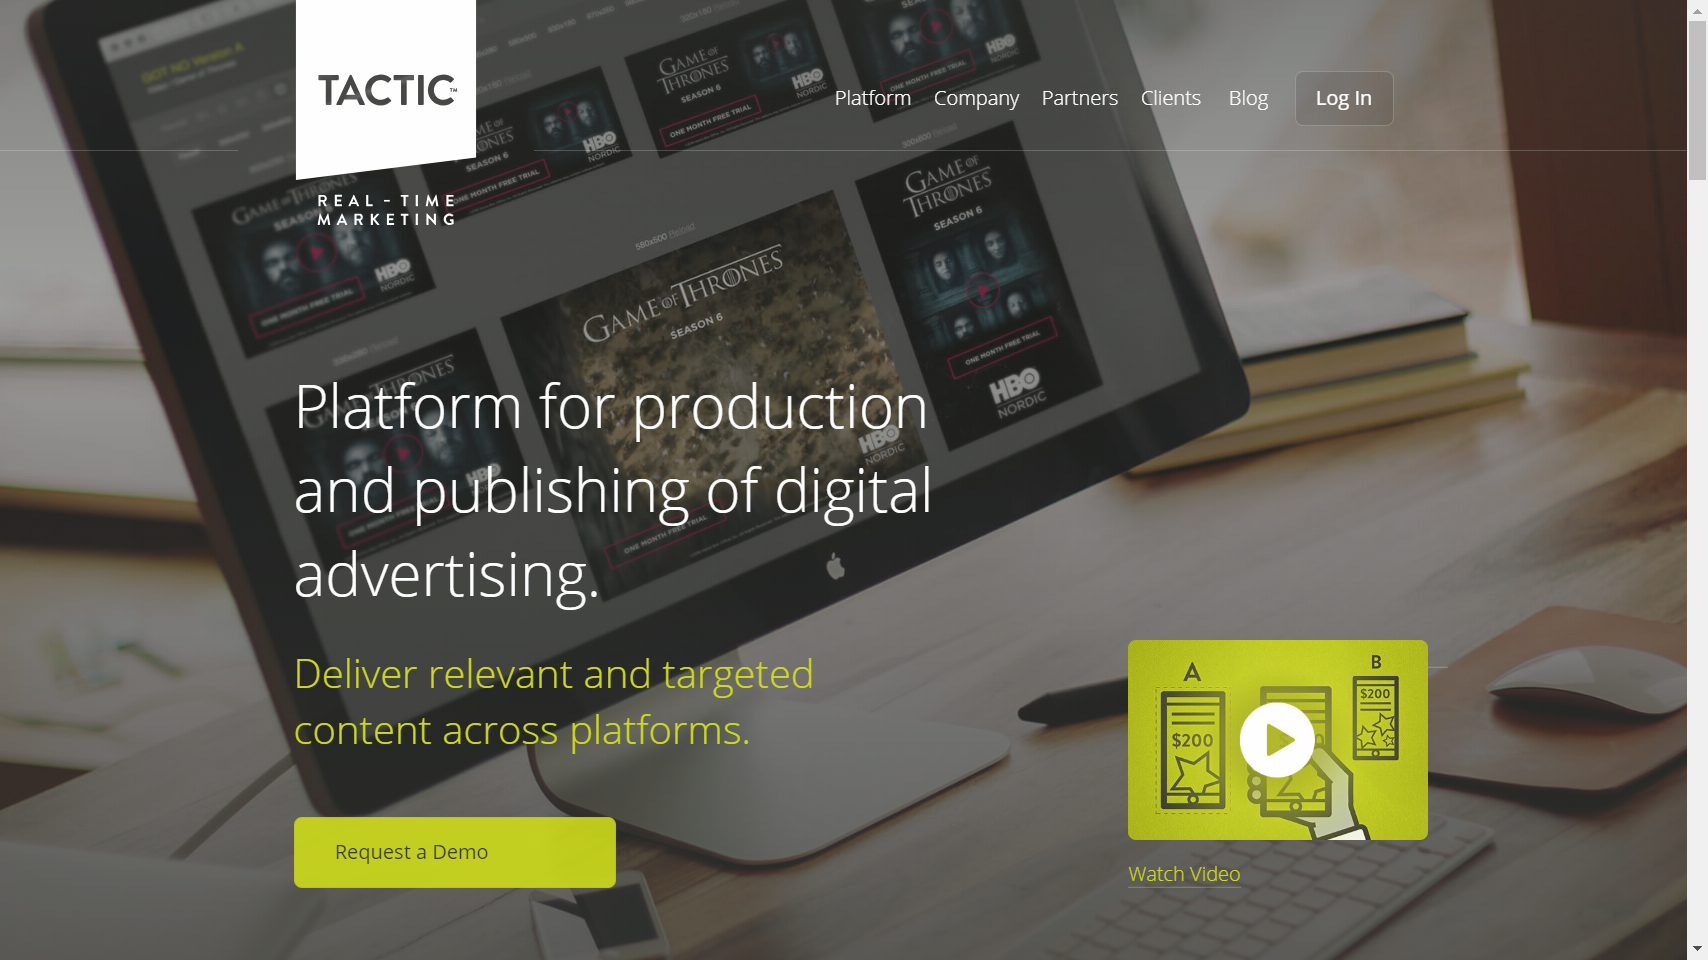
\includegraphics[width=\textwidth]{line/tacticrealtime_com_(1366x768).png}
    \caption{tacticrealtime.com}
    \label{fig:competitors-tacticrealtime.com}
\end{figure}

\subsubsection{Forside og undersider}

Forsiden består av bakgrunnsbilde som inneholder logo, meny, overskrifter og en video.  
Deretter kommer det litt tekst om firmaet, informasjon om plattformen, logo av ledende  Ad-servers og DSP's, partnerprogram og utvalgte kunder. Siden avsluttes med en \q{Contact us}-seksjon.

Nettstedet består også av følgende undersider:
\begin{itemize}
\item Platform
\item Company
\item Partners
\item Clients
\item Blog
\end{itemize}

\subsubsection{Teknisk analyse}
Bruke google lighthouse

\subsubsection{Styrker}
Førsteinntrykket er bra. Nettstedet fremstår som profesjonelt, noe som styrker inntrykket av bedriften. Nettstedet har også god oppbygning og struktur. 
Sterk profil. Det er ganske tydelig at grønn er pimærfargen til selskapet.

\subsubsection{Svakheter}
Hele nettstedet er på engelsk i tillegg til at det er et .com-domene. Dette kan forvirre brukerne. Vanskelig å skjønne at dette er et firma som er lokalisert i Oslo. En annen svakhet er at det er lite luft rundt noen elementer, som fører til at nettstedet fremstår som kompakt og mer rotete. Det er heller ikke samme mengde luft over og under elementene. Dette er også med på å trekke ned helhetsinntrykket. Det er heller ikke mulig å bevege seg rundt på nettstedet ved hjelp av tastaturet. Dette gjør det også vanskelig å navigere seg rundt ved hjelp av skjermleser, noe som er et krav i loven om universell utforming og tilgjengelighet. I tillegg får nettstedet mange kontrastfeil, som også bryter lovkravet om universell utforming.

\subsection{Marketer Technologies AS}
Nettstedet til Marketer Technologies AS ligger på følgende domene;
https://marketer.tech/

\subsubsection{Førsteinntrykk}
Førsteinntrykket av nettstedet er positivt, fordi den fremstår som ryddig og profesjonell. Det første som møter deg er headeren til nettstedet, som inneholder logoen til firmaet og en meny. Under menyen er en tittel, en underoverskrift og to lenker. Får også opp et ikon for chat. Det at man enkelt kan ta kontakt kan for en kunde virke betryggende, og kan være med å øke troverdigheten til bedriften.

\begin{figure}[H]
    \centering
    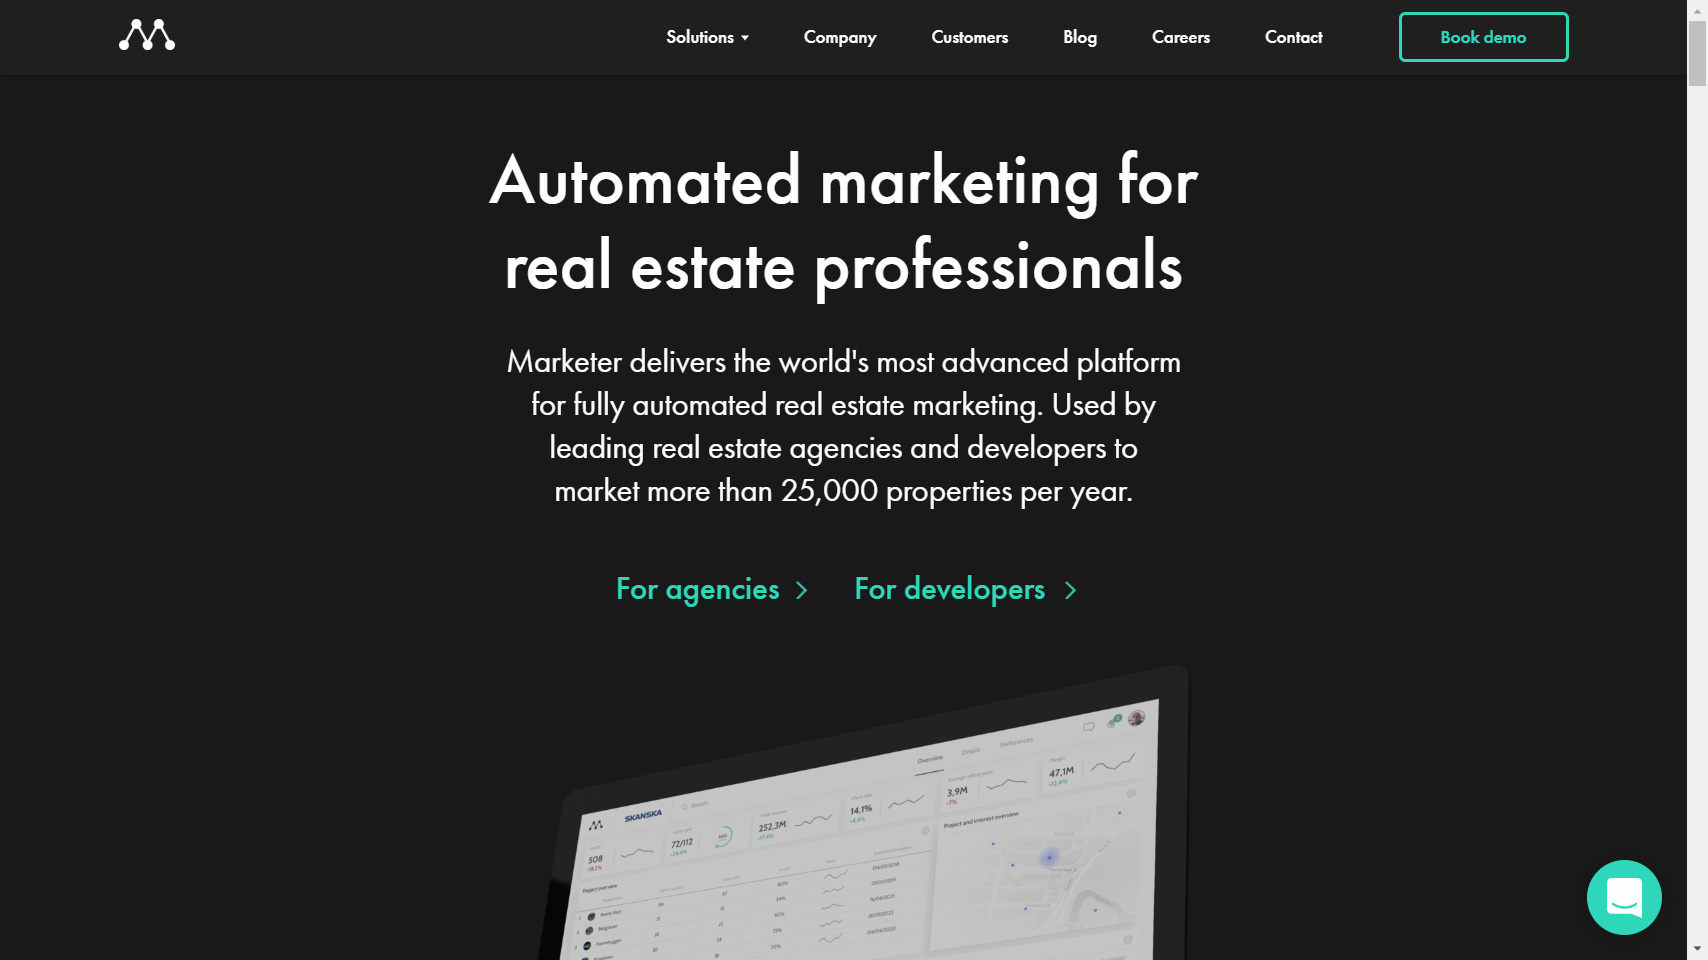
\includegraphics[width=\textwidth]{line/marketer_tech_(1366x768).png}
    \caption{marketer.tech}
    \label{fig:competitors-marketer.tech}
\end{figure}

\subsubsection{Forside og undersider}

Forsiden, i tillegg til headeren, består av logo til noen utvalgre kunder, prosessen til Marketer, animasjoner, resultater fra tidligere prosjekter og en presentasjon av deres løsninger. Helt nederst på siden kommer bunnfeltet, der organisasjonsnummeret, kontaktinformasjon og adresse blir presentert.

Nettstedet består også av følgende undersider:
\begin{itemize}
\item Solutions
\item Company
\item Customers
\item Blog
\item Careers 
\item Contact
\item Book demo
\end{itemize}

\subsubsection{Teknisk analyse}
5 kontrastfeil. Hele 147 feil når det kommer til universell utforming og tilgjengelighet. 135 av disse feilene er manglende bruk av alt-tekster.

\subsubsection{Styrker}
Bra førsteinntrykk. Nettsted som skiller seg ut og er gjennomført. Chat som forenkler kontakt-prosessen for kunder. Klar og tydelig profil. Marketer har åpenbart sort som primærfarge og turkis som aksentfarge

\subsubsection{Svakheter}
Stort og tregt nettsted. Mange feil når det gjelder universell utforming og tilgjengelighet.


\subsection{Inviso AS}
Nettstedet til Inviso AS ligger på følgende domene;
https://www.inviso.no/

\subsubsection{Førsteinntrykk}
Førsteinntrykket av nettstedet er at den fremstår som rotete. Hovedgrunnen til dette er at det er mange elementer og mye som skjer i headeren\footnote{Hodet til nettstedet}. Logoen og noe av teksten på bakgrunnsbilde er også vanskelig å se, på grunn av for dårlig kontrast. 

\begin{figure}[H]
    \centering
    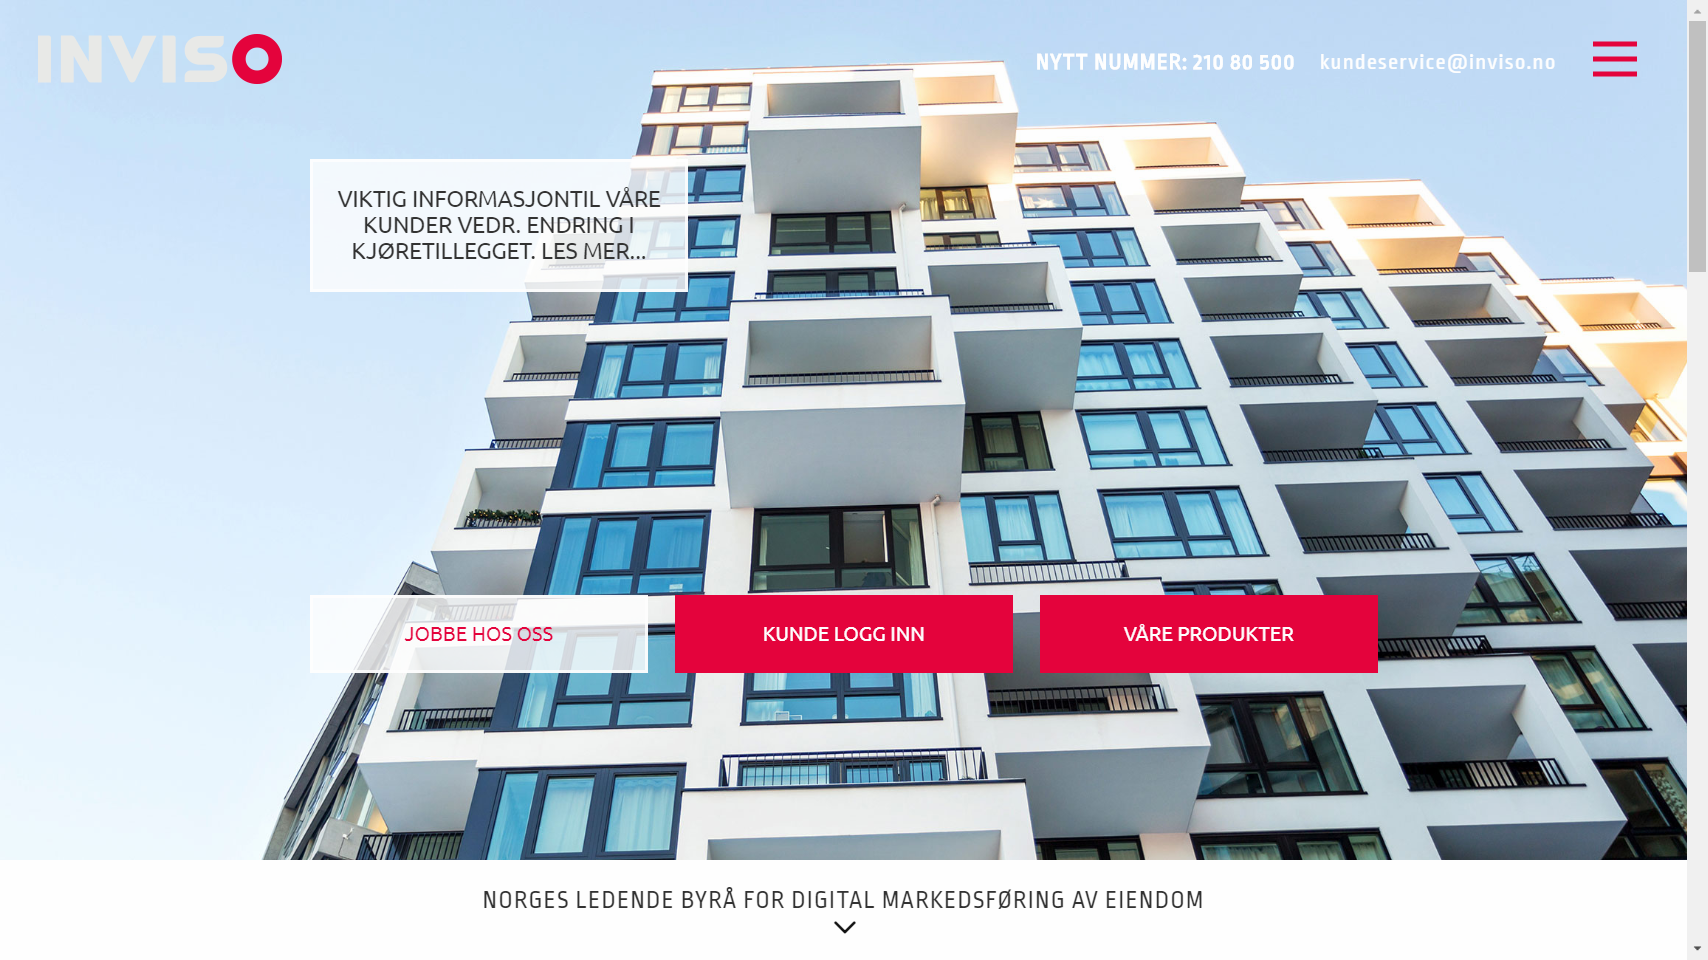
\includegraphics[width=\textwidth]{line/inviso_no_(1366x768).png}
    \caption{inviso.no}
    \label{fig:competitors-inviso.no}
\end{figure}

\subsubsection{Forside og undersider}
I tillegg til headeren består forsiden av \q{Om oss}-tekst, deres tjenester og utvalgte kunder. 

Nettstedet består også av følgende undersider:
\begin{itemize}
\item Inviso
\item Våre produkter
\item Kontakt
\item Galleri
\item Verktøy
\item Nyheter
\end{itemize}


\subsubsection{Teknisk analyse}
4 kontrastfeil. 17 bilder som mangler alt-tekst. 

\subsubsection{Styrker}
Bra profil. Man skjønner lett at rød er primærfargen til Inviso.
Det tekstlige innholdet på siden er bra skrevet.

\subsubsection{Svakheter}
For mye informasjon i headeren. En stor svakhet er at nettstedet får mange feil når man kjører tester når det gjelder universell utforming og tilgjengelighet. Har mobil-meny på fullversjon av siden.

\subsection{Konklusjon}
Felles for alle 3 konkurrentene er at ingen av de følger loven om universell utforming og tilgjengelighet.

En annen ting alle har til felles er at de presenterer sine kunder og/eller partnere. Dette er noe Sirkus Media burde også burde gjøre. Det er tillitsvekkende og fører til bedre troverdighet.

Som vi kan se i figur \ref{fig:competitors-mobile} har alle konkurrentene gått for samme løsning når det kommer til design på mobil. Alle 3 har logo oppe til venstre, og et meny ikon til høyre.
Dette er noe vi burde løse annerledes. Undersøkelser \footnote{Kilde: Luke Wroblewski, en internasjonalt anerkjent brukeropplevelsesdesigner \url{https://www.lukew.com/ff/entry.asp?1945}} viser at dette er langt fra beste løsning.

\begin{figure}[bh]
    \begin{center}
        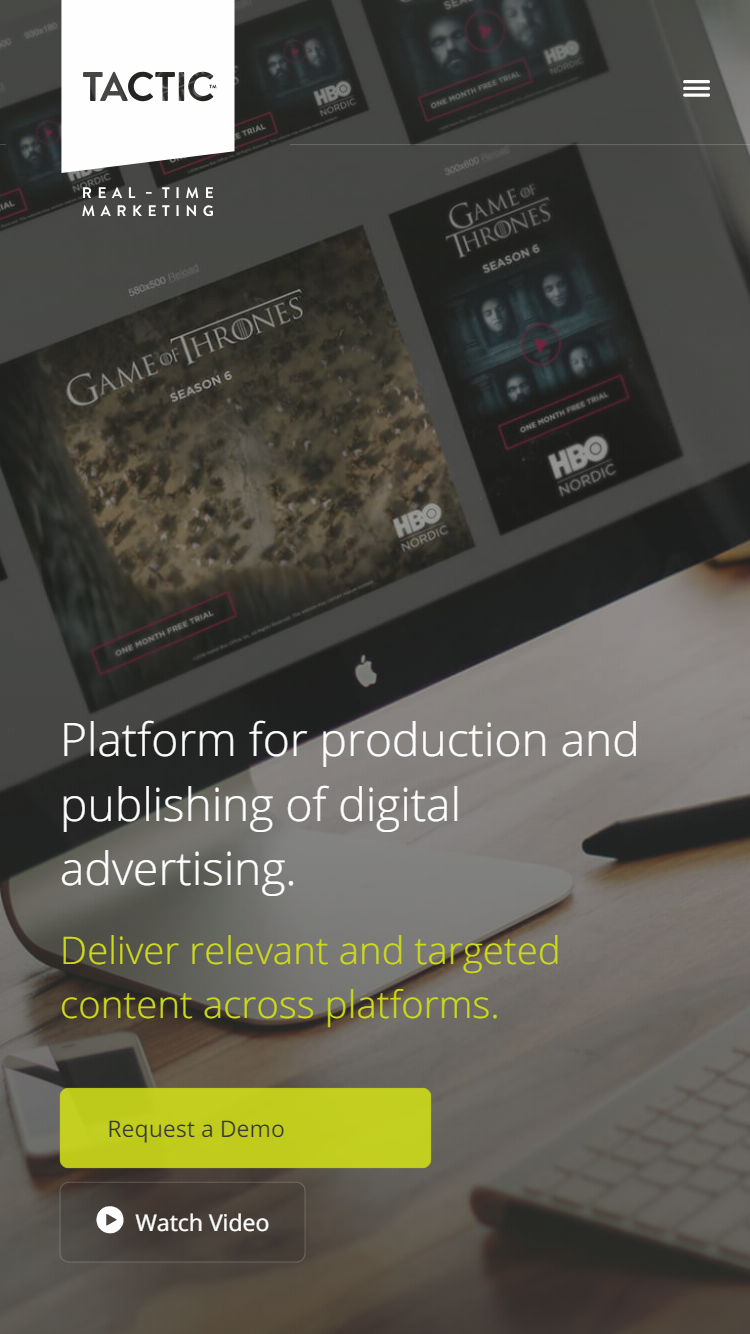
\includegraphics[width=0.3\textwidth]{line/tacticrealtime_com_(iPhone_6_7_8).png}
        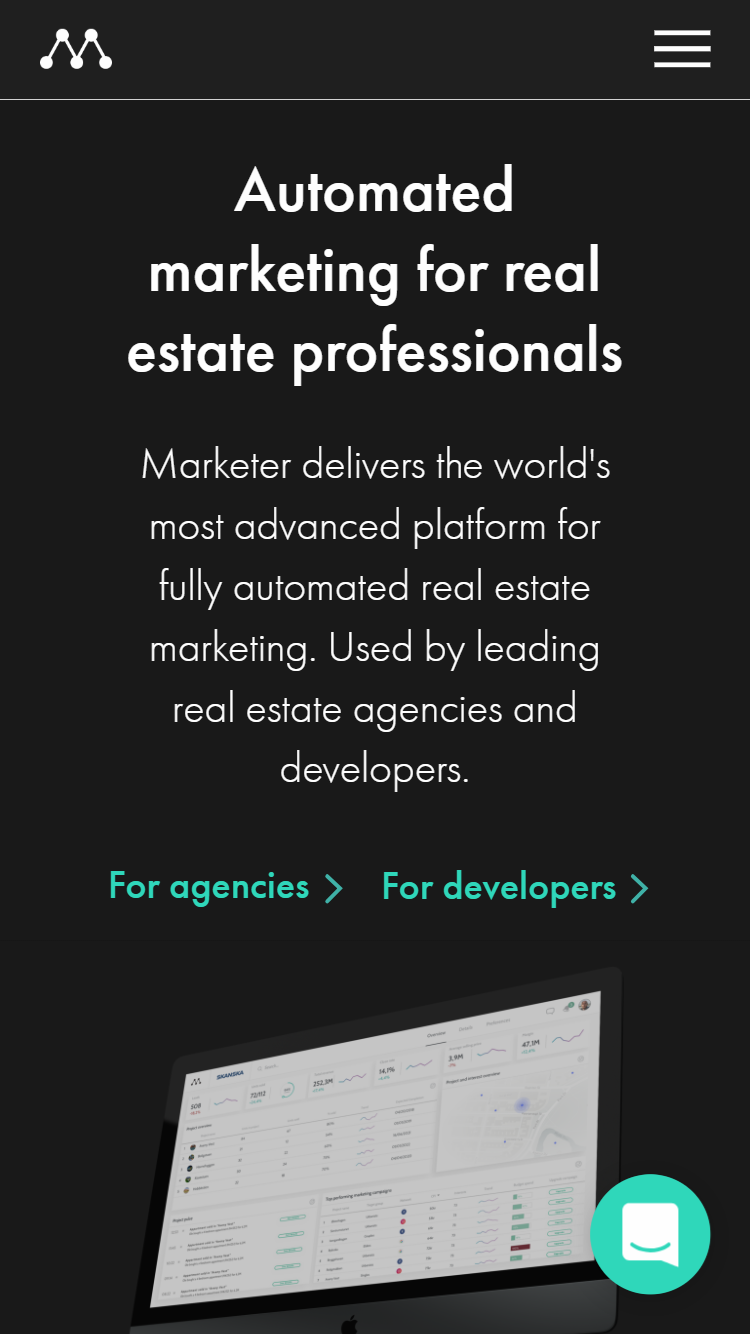
\includegraphics[width=0.3\textwidth]{line/marketer_tech_(iPhone_6_7_8).png}
        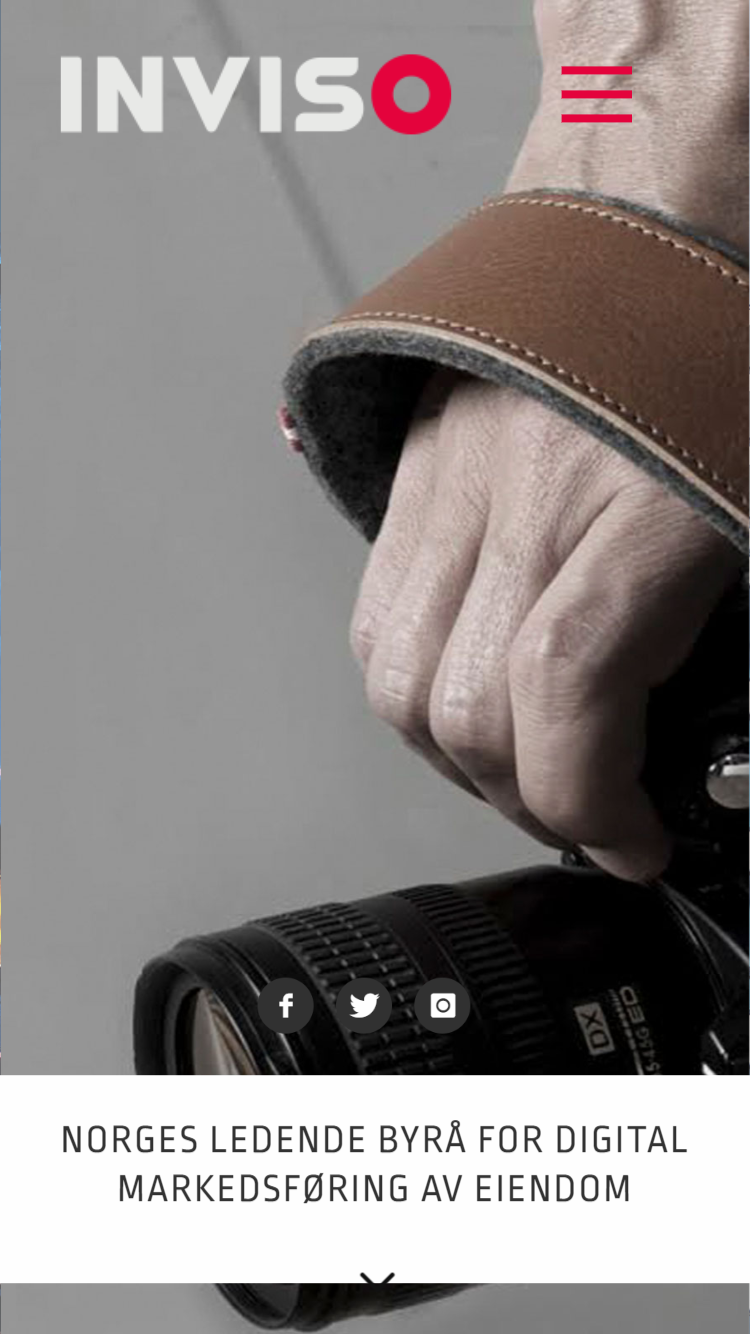
\includegraphics[width=0.3\textwidth]{line/inviso_no_(iPhone_6_7_8).png}
        \caption{Mobil sider}
        \label{fig:competitors-mobile}
    \end{center}
\end{figure}

\begin{figure}[H]
    \begin{center}
        \subfigure[tacticrealtime.com]{\label{fig:competitors-lighthouse-summary-tacticrealtime.com}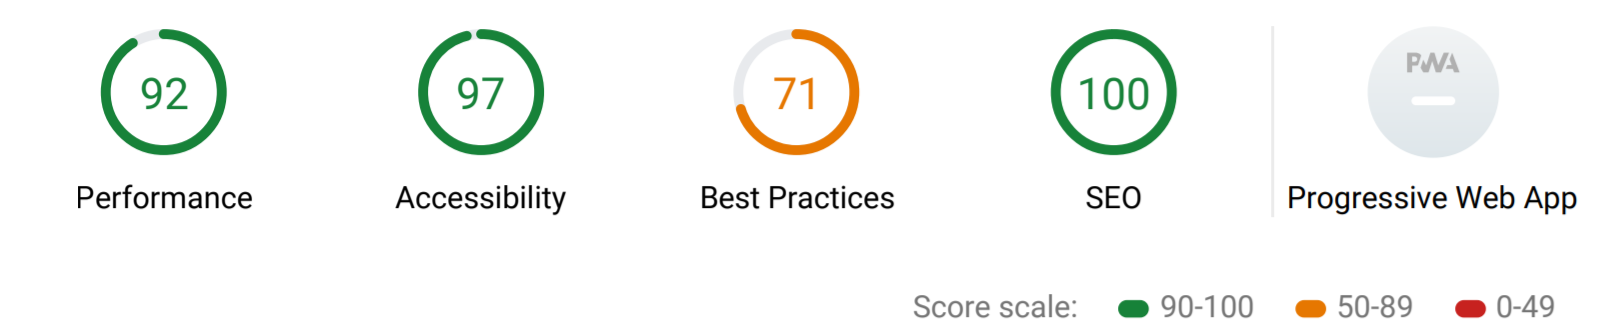
\includegraphics[width=\textwidth]{line/tacticrealtime_com-lighthouse.png}}
        \subfigure[marketer.tech]{\label{fig:competitors-lighthouse-summary-marketer.tech}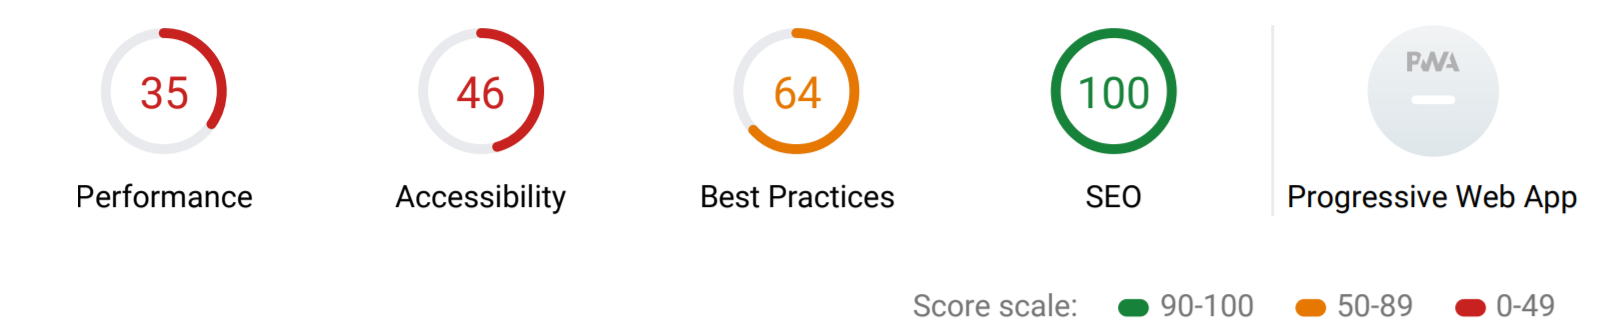
\includegraphics[width=\textwidth]{line/marketer_tech-lighthouse.png}}
        \subfigure[inviso.no]{\label{fig:competitors-lighthouse-summary-inviso.no}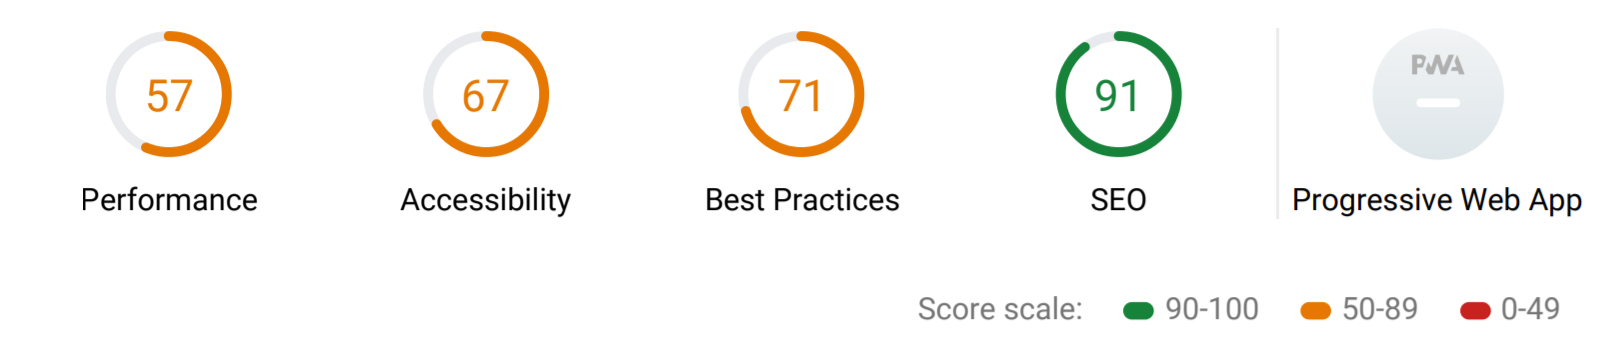
\includegraphics[width=\textwidth]{line/inviso_no-lighthouse.png}}
        \caption{Lighthouse test resultater}
        \label{fig:competitors-lighthouse-summary}
    \end{center}
\end{figure}

Figur \ref{fig:competitors-lighthouse-summary} viser test resultater fra Google Lighthouse. Se vedlegg X for full rapport på hver av disse. Merk at PWA ikke viser resultat som den skal, men det gjør ingenting ettersom det ikke er så relevant for disse nettstedene uansett \footnote{Se avsnitt \ref{sec:analysis-current-lighthouse} for informasjon om hvorfor}.
Vi har satt oss som mål å få minst like bra score som gjennomsnittet til disse.

\clearpage